\documentclass[11pt,a4paper]{article}

% ---------------------------------------------------------------
% Tipografia: Palatino, versalete, uma cor de destaque (bord\^o)
% Mesmo pre\^ambulo da lista de termologia.
% ---------------------------------------------------------------
\usepackage[utf8]{inputenc}
\usepackage[T1]{fontenc}
\usepackage[brazil]{babel}
\usepackage[sc,osf]{mathpazo}
\usepackage{microtype}
\usepackage[top=2.4cm, bottom=2.6cm, left=2.6cm, right=2.6cm]{geometry}
\usepackage{amsmath}
\usepackage{amssymb}
\usepackage{xcolor}
\usepackage{tcolorbox}
\tcbuselibrary{skins, breakable}
\usepackage{enumitem}
\usepackage{booktabs}
\usepackage{array}
\usepackage{needspace}
\usepackage{hyperref}
\usepackage{graphicx}
\graphicspath{{figuras/}}

\definecolor{vinho}{RGB}{122, 27, 42}
\definecolor{grafite}{RGB}{70, 70, 70}
\hypersetup{colorlinks=true, linkcolor=vinho, urlcolor=vinho}

\linespread{1.06}
\setlength{\parindent}{0pt}
\setlength{\parskip}{0.45em}

% ---------------------------------------------------------------
% Formata\c{c}\~ao das quest\~oes
% ---------------------------------------------------------------
\newcommand{\fonte}[1]{{\small\scshape\color{grafite}#1}}
\newcommand{\enem}[3]{\fonte{ENEM #1 \,\textperiodcentered\, #2 \,\textperiodcentered\, Q#3}}

\newenvironment{questao}[2]{%
  \needspace{6\baselineskip}
  \par\addvspace{1.6em}
  {\large\bfseries\color{vinho}Quest\~ao #1}\hfill #2\\[-0.55em]
  {\color{black!25}\rule{\linewidth}{0.4pt}}
  \par\nobreak\smallskip
}{\par\addvspace{0.4em}}

\newcommand{\parte}[1]{%
  \needspace{7\baselineskip}
  \vspace{1.8em}
  {\Large\bfseries #1}\\[-0.55em]
  {\color{black!30}\rule{\linewidth}{0.5pt}}
  \par\nobreak\smallskip
}

\newtcolorbox{painel}{blanker, breakable, left=12pt,
  borderline west={1.4pt}{0pt}{black!30},
  before skip=11pt, after skip=11pt}

% figura recortada do caderno oficial do INEP
\newcommand{\figuraoriginal}[2]{%
  \begin{center}
    \includegraphics[width=#1]{#2}
  \end{center}}

% refer\^encia bibliogr\'afica do enunciado, como na prova
\newcommand{\fontebib}[1]{{\raggedleft\scriptsize\color{grafite}#1\par}}

% alternativas nunca se separam entre paginas
\setlist[enumerate,1]{label=\textbf{\Alph*)}, leftmargin=2em, nosep,
  beginpenalty=10000, midpenalty=10000}

% ---------------------------------------------------------------
\begin{document}
% ---------------------------------------------------------------

\thispagestyle{empty}

{\scshape\color{vinho}cursinho solid\'ario \,\textperiodcentered\, f\'isica}\\[-0.5em]
{\color{vinho}\rule{\linewidth}{1.6pt}}\\[0.9em]
{\huge\bfseries Lista de Quest\~oes}\\[0.35em]
{\LARGE Ondas, Som e Luz}\\[0.7em]
\hfill {\color{grafite}2026}\\[-0.3em]
{\color{black!30}\rule{\linewidth}{0.5pt}}

\vspace{1.0em}

\begin{painel}
\begin{itemize}[nosep, leftmargin=1.5em]
  \item A lista segue a ordem da aula: o que \'e onda, fen\^omenos
        ondulat\'orios, ac\'ustica, luz e vis\~ao, espelhos.
  \item Comece por Q2, Q5 e Q14: uma de ondas, uma de fen\^omenos e uma de
        espelhos. No fim tem o gabarito comentado.
\end{itemize}
\end{painel}

\newpage

{\renewcommand{\arraystretch}{1.2}
\begin{tabular}{@{}cll@{}}
  \multicolumn{3}{@{}l}{{\scshape\color{vinho}mapa da lista}}\\
  \addlinespace[2pt]
  \toprule
  \# & Origem & Tema \\
  \midrule
  1  & ENEM 2025 \,\textperiodcentered\, Q126   & Espectro: controle de TV e de drone \\
  2  & ENEM 2023 \,\textperiodcentered\, Q91    & Telefone de lata: o que diminui \\
  3  & ENEM 2023 \,\textperiodcentered\, Q115   & Celular no avi\~ao: mesma frequ\^encia \\
  \midrule
  4  & ENEM 2023 \,\textperiodcentered\, Q92    & Difra\c{c}\~ao e o laser de CD, DVD e Blu-ray \\
  5 & ENEM 2020 \,\textperiodcentered\, Q94    & Fone com cancelamento de ru\'ido \\
  6 & ENEM 2025 \,\textperiodcentered\, Q128   & Carro el\'etrico e r\'adio AM \\
  \midrule
  7 & ENEM 2021 \,\textperiodcentered\, Q134   & Sino dos ventos: frequ\^encia e velocidade \\
  8 & ENEM 2024 \,\textperiodcentered\, Q130   & Efeito Doppler: sirene e radar \\
  \midrule
  9 & ENEM 2021 \,\textperiodcentered\, Q115   & Cor das folhas e cores complementares \\
  10 & ENEM 2022 \,\textperiodcentered\, Q101   & Cones e bastonetes \\
  11 & ENEM 2012 \,\textperiodcentered\, Q64    & Pesca com lan\c{c}a: refra\c{c}\~ao \\
  12 & ENEM 2022 \,\textperiodcentered\, Q96    & ``Luz engarrafada'' \\
  13 & ENEM 2019 \,\textperiodcentered\, Q132   & Vis\~ao debaixo d'\'agua \\
  \midrule
  14 & ENEM 2024 \,\textperiodcentered\, Q131   & Mirasc\'opio: imagem real \\
  \bottomrule
\end{tabular}}

\newpage

% ===================================================================
\parte{Parte I --- O Que \'E Onda}
% ===================================================================

\begin{questao}{1}{\enem{2025}{caderno amarelo}{126}}
Alguns aparelhos do nosso cotidiano, como TVs e drones, s\~ao operados a
dist\^ancia por controle remoto. A diferen\c{c}a no sistema de controle
desses aparelhos se d\'a em rela\c{c}\~ao \`a radia\c{c}\~ao emitida, pois, nas TVs,
o acionamento do controle remoto deve ser realizado a uma curta dist\^ancia
e o sistema receptor de sinal n\~ao pode estar obstru\'ido. Por outro lado,
nos drones, o sistema de controle funciona a dist\^ancias relativamente
grandes, da ordem de alguns quil\^ometros.

O acionamento dos equipamentos citados corresponde \`a emiss\~ao de ondas,
respectivamente, nas regi\~oes
\begin{enumerate}
  \item vis\'ivel e raios X.
  \item r\'adio e ultravioleta.
  \item ultravioleta e vis\'ivel.
  \item infravermelho e r\'adio.
  \item raios X e infravermelho.
\end{enumerate}
\end{questao}

\begin{questao}{2}{\enem{2023}{caderno amarelo}{91}}
Na tirinha de Mauricio de Sousa, os personagens Cebolinha e Casc\~ao fazem
uma brincadeira utilizando duas latas e um barbante. Ao perceberem que o
som pode ser transmitido atrav\'es do barbante, resolvem alterar o
comprimento do barbante para ficar cada vez mais extenso. As demais
condi\c{c}\~oes permaneceram inalteradas durante a brincadeira.

\figuraoriginal{0.92\linewidth}{enem2023_q091_tirinha}

Na pr\'atica, \`a medida que se aumenta o comprimento do barbante, ocorre a
redu\c{c}\~ao de qual caracter\'istica da onda sonora?
\begin{enumerate}
  \item Altura.
  \item Per\'iodo.
  \item Amplitude.
  \item Velocidade.
  \item Comprimento de onda.
\end{enumerate}
\end{questao}

\begin{questao}{3}{\enem{2023}{caderno amarelo}{115}}
\'E comum em viagens de avi\~ao sermos solicitados a desligar aparelhos cujo
funcionamento envolva a emiss\~ao ou a recep\c{c}\~ao de ondas
eletromagn\'eticas, como celulares. A justificativa dada para esse
procedimento \'e, entre outras coisas, a necessidade de eliminar fontes de
sinais eletromagn\'eticos que possam interferir nas comunica\c{c}\~oes, via
r\'adio, dos pilotos com a torre de controle.

Essa interfer\^encia poder\'a ocorrer somente se as ondas emitidas pelo
celular e as recebidas pelo r\'adio do avi\~ao
\begin{enumerate}
  \item forem ambas aud\'iveis.
  \item tiverem a mesma pot\^encia.
  \item tiverem a mesma frequ\^encia.
  \item tiverem a mesma intensidade.
  \item propagarem-se com velocidades diferentes.
\end{enumerate}
\end{questao}

% ===================================================================
\parte{Parte II --- Fen\^omenos Ondulat\'orios}
% ===================================================================

\begin{questao}{4}{\enem{2023}{caderno amarelo}{92}}
Informa\c{c}\~oes digitais --- dados --- s\~ao gravadas em discos \'opticos,
como CD e DVD, na forma de cavidades microsc\'opicas. A grava\c{c}\~ao e a
leitura \'optica dessas informa\c{c}\~oes s\~ao realizadas por um laser (fonte
de luz monocrom\'atica). Quanto menores as dimens\~oes dessas cavidades,
mais dados s\~ao armazenados na mesma \'area do disco. O fator limitante para
a leitura de dados \'e o espalhamento da luz pelo efeito de difra\c{c}\~ao,
fen\^omeno que ocorre quando a luz atravessa um obst\'aculo com dimens\~oes
da ordem de seu comprimento de onda. Essa limita\c{c}\~ao motivou o
desenvolvimento de lasers com emiss\~ao em menores comprimentos de onda,
possibilitando armazenar e ler dados em cavidades cada vez menores.

Em qual regi\~ao espectral se situa o comprimento de onda do laser que
otimiza o armazenamento e a leitura de dados em discos de uma mesma \'area?
\begin{enumerate}
  \item Violeta.
  \item Azul.
  \item Verde.
  \item Vermelho.
  \item Infravermelho.
\end{enumerate}
\end{questao}

\begin{questao}{5}{\enem{2020}{caderno amarelo}{94}}
Os fones de ouvido tradicionais transmitem a m\'usica diretamente para os
nossos ouvidos. J\'a os modelos dotados de tecnologia redutora de ru\'ido
--- Cancelamento de Ru\'ido (CR) --- al\'em de transmitirem m\'usica, tamb\'em
reduzem todo ru\'ido inconsistente \`a nossa volta, como o barulho de
turbinas de avi\~ao e aspiradores de p\'o. Os fones de ouvido CR n\~ao reduzem
realmente barulhos irregulares como discursos e choros de beb\^es. Mesmo
assim, a supress\~ao do ronco das turbinas do avi\~ao contribui para reduzir
a ``fadiga de ru\'ido'', um cansa\c{c}o persistente provocado pela exposi\c{c}\~ao
a um barulho alto por horas a fio. Esses aparelhos tamb\'em permitem que
n\'os ou\c{c}amos m\'usicas ou assistamos a v\'ideos no trem ou no avi\~ao a um
volume muito menor (e mais seguro).

\fontebib{Dispon\'ivel em: http://tecnologia.uol.com.br. Acesso em: 21 abr. 2015 (adaptado).}

A tecnologia redutora de ru\'ido CR utilizada na produ\c{c}\~ao de fones de
ouvido baseia-se em qual fen\^omeno ondulat\'orio?
\begin{enumerate}
  \item Absor\c{c}\~ao.
  \item Interfer\^encia.
  \item Polariza\c{c}\~ao.
  \item Reflex\~ao.
  \item Difra\c{c}\~ao.
\end{enumerate}
\end{questao}

\begin{questao}{6}{\enem{2025}{caderno amarelo}{128}}
{\centering\bfseries Carros el\'etricos p\~oem fim ao longo reinado da r\'adio AM\par}

As montadoras de autom\'oveis est\~ao em uma corrida rumo a um futuro
eletrificado, e r\'adios AM est\~ao ficando pelo caminho. O problema, dizem
os especialistas, \'e que os motores dos ve\'iculos el\'etricos geram
frequ\^encias eletromagn\'eticas do mesmo comprimento de onda que os sinais
das r\'adios AM. ``Voc\^e tem dois sinais que colidem um com o outro e se
cancelam'', disse o diretor de inova\c{c}\~ao de motores e tecnologia de uma
fabricante de autope\c{c}as.

\fontebib{Dispon\'ivel em: www1.folha.uol.com.br. Acesso em: 20 nov. 2018 (adaptado).}

O problema mencionado refere-se a qual fen\^omeno ondulat\'orio?
\begin{enumerate}
  \item Difra\c{c}\~ao.
  \item Reflex\~ao.
  \item Refra\c{c}\~ao.
  \item Resson\^ancia.
  \item Interfer\^encia.
\end{enumerate}
\end{questao}

% ===================================================================
\parte{Parte III --- Ac\'ustica}
% ===================================================================

\begin{questao}{7}{\enem{2021}{caderno amarelo}{134}}
O sino dos ventos \'e composto por v\'arias barras met\'alicas de mesmo
material e espessura, mas de comprimentos diferentes, conforme a figura.

\figuraoriginal{0.34\linewidth}{enem2021_q134_sino}

Considere $f_1$ e $v_1$, respectivamente, como a frequ\^encia fundamental e a
velocidade de propaga\c{c}\~ao do som emitido pela barra de menor comprimento,
e $f_2$ e $v_2$ s\~ao essas mesmas grandezas para o som emitido pela barra de
maior comprimento.

As rela\c{c}\~oes entre as frequ\^encias fundamentais e entre as velocidades de
propaga\c{c}\~ao s\~ao, respectivamente,
\begin{enumerate}
  \item $f_1 < f_2$ e $v_1 < v_2$.
  \item $f_1 < f_2$ e $v_1 = v_2$.
  \item $f_1 < f_2$ e $v_1 > v_2$.
  \item $f_1 > f_2$ e $v_1 = v_2$.
  \item $f_1 > f_2$ e $v_1 > v_2$.
\end{enumerate}
\end{questao}

\begin{questao}{8}{\enem{2024}{caderno cinza}{130}}
Uma ambul\^ancia em alta velocidade com a sirene ligada desloca-se em
dire\c{c}\~ao a um radar operado por uma pessoa. O radar emite ondas de
r\'adio com frequ\^encia $f_0$ que s\~ao refletidas pela dianteira da
ambul\^ancia, retornando para o detector com frequ\^encia $f_r$. A
percep\c{c}\~ao do operador do radar, em rela\c{c}\~ao ao som emitido pela
sirene, \'e de que este se altera \`a medida que a ambul\^ancia se aproxima ou
se afasta.

Durante a aproxima\c{c}\~ao, como o operador percebe o som da sirene e qual \'e
a rela\c{c}\~ao entre as frequ\^encias $f_r$ e $f_0$ medidas pelo radar?
\begin{enumerate}
  \item Mais grave do que o som emitido e $f_r < f_0$.
  \item Mais agudo do que o som emitido e $f_r < f_0$.
  \item Mais agudo do que o som emitido e $f_r = f_0$.
  \item Mais agudo do que o som emitido e $f_r > f_0$.
  \item Mais grave do que o som emitido e $f_r > f_0$.
\end{enumerate}
\end{questao}

% ===================================================================
\parte{Parte IV --- Luz, Cor e Vis\~ao}
% ===================================================================

\begin{questao}{9}{\enem{2021}{caderno amarelo}{115}}
No outono, as folhas das \'arvores mudam de cor, de verde para tons de
amarelo, castanho, laranja e vermelho. A cor verde das folhas deve-se ao
pigmento clorofila. Nas plantas de folhas caducas, a produ\c{c}\~ao de
clorofila diminui e o tom verde desvanece, permitindo assim que outros
pigmentos, como o caroteno, de colora\c{c}\~ao amarelo-alaranjado, e a
antocianina, de tons avermelhados, passem a dominar a tonalidade das
folhas. A colora\c{c}\~ao observada se d\'a em fun\c{c}\~ao da intera\c{c}\~ao desses
pigmentos com a radia\c{c}\~ao solar.

Conforme apresentado no espectro de absor\c{c}\~ao, as mol\'eculas de
clorofila absorvem a radia\c{c}\~ao solar nas regi\~oes do azul e do vermelho,
assim a luz refletida pelas folhas tem falta desses dois tons e as vemos na
cor verde. J\'a as antocianinas absorvem a luz desde o azul at\'e o verde.
Nesse caso, a luz refletida pelas folhas que cont\^em antocianinas aparece
conforme as cores complementares, ou seja, vermelho-alaranjado.

\figuraoriginal{\linewidth}{enem2021_q115_espectro}

Em qual faixa do espectro vis\'ivel os carotenos absorvem majoritariamente?
\begin{enumerate}
  \item Entre o violeta e o azul.
  \item Entre o azul e o verde.
  \item Entre o verde e o amarelo.
  \item Entre o amarelo e o laranja.
  \item Entre o laranja e o vermelho.
\end{enumerate}
\end{questao}

\begin{questao}{10}{\enem{2022}{caderno amarelo}{101}}
No processo de capta\c{c}\~ao da luz pelo olho para a forma\c{c}\~ao de imagens
est\~ao envolvidas duas estruturas celulares: os cones e os bastonetes. Os
cones s\~ao sens\'iveis \`a energia dos f\'otons, e os bastonetes, \`a
quantidade de f\'otons incidentes. A energia dos f\'otons que comp\~oem os
raios luminosos est\'a associada \`a sua frequ\^encia, e a intensidade, ao
n\'umero de f\'otons incidentes.

Um animal que tem bastonetes mais sens\'iveis ir\'a
\begin{enumerate}
  \item apresentar daltonismo.
  \item perceber cores fora do espectro do vis\'ivel.
  \item enxergar bem em ambientes mal iluminados.
  \item necessitar de mais luminosidade para enxergar.
  \item fazer uma pequena distin\c{c}\~ao de cores em ambientes iluminados.
\end{enumerate}
\end{questao}

\begin{questao}{11}{\enem{2012}{1\textordmasculine{} dia, caderno azul}{64}}
Alguns povos ind\'igenas ainda preservam suas tradi\c{c}\~oes realizando a
pesca com lan\c{c}as, demonstrando uma not\'avel habilidade. Para fisgar um
peixe em um lago com \'aguas tranquilas o \'indio deve mirar abaixo da
posi\c{c}\~ao em que enxerga o peixe.

Ele deve proceder dessa forma porque os raios de luz
\begin{enumerate}
  \item refletidos pelo peixe n\~ao descrevem uma trajet\'oria retil\'inea no
        interior da \'agua.
  \item emitidos pelos olhos do \'indio desviam sua trajet\'oria quando passam
        do ar para a \'agua.
  \item espalhados pelo peixe s\~ao refletidos pela superf\'icie da \'agua.
  \item emitidos pelos olhos do \'indio s\~ao espalhados pela superf\'icie da
        \'agua.
  \item refletidos pelo peixe desviam sua trajet\'oria quando passam da \'agua
        para o ar.
\end{enumerate}
\end{questao}

\begin{questao}{12}{\enem{2022}{caderno amarelo}{96}}
Em 2002, um mec\^anico da cidade mineira de Uberaba (MG) teve uma ideia para
economizar o consumo de energia el\'etrica e iluminar a pr\'opria casa num dia
de sol. Para isso, ele utilizou garrafas pl\'asticas PET com \'agua e cloro,
conforme ilustram as figuras. Cada garrafa foi fixada ao telhado de sua casa
em um buraco com di\^ametro igual ao da garrafa, muito maior que o
comprimento de onda da luz. Nos \'ultimos dois anos, sua ideia j\'a alcan\c{c}ou
diversas partes do mundo e deve atingir a marca de 1 milh\~ao de casas
utilizando a ``luz engarrafada''.

\figuraoriginal{0.62\linewidth}{enem2022_q096_garrafa}

Que fen\^omeno \'optico explica o funcionamento da ``luz engarrafada''?
\begin{enumerate}
  \item Difra\c{c}\~ao.
  \item Absor\c{c}\~ao.
  \item Polariza\c{c}\~ao.
  \item Reflex\~ao.
  \item Refra\c{c}\~ao.
\end{enumerate}
\end{questao}

\begin{questao}{13}{\enem{2019}{caderno azul}{132}}
A maioria das pessoas fica com a vis\~ao emba\c{c}ada ao abrir os olhos
debaixo d'\'agua. Mas h\'a uma exce\c{c}\~ao: o povo moken, que habita a costa da
Tail\^andia. Essa caracter\'istica se deve principalmente \`a adaptabilidade
do olho e \`a plasticidade do c\'erebro, o que significa que voc\^e tamb\'em,
com algum treinamento, poderia enxergar relativamente bem debaixo d'\'agua.
Estudos mostraram que as pupilas de olhos de indiv\'iduos moken sofrem
redu\c{c}\~ao significativa debaixo d'\'agua, o que faz com que os raios luminosos
incidam quase paralelamente ao eixo \'optico da pupila.

\fontebib{GISL\'EN, A. et al. Visual Training Improves Underwater Vision in
Children. \textbf{Vision Research}, n. 46, 2006 (adaptado).}

A acuidade visual associada \`a redu\c{c}\~ao das pupilas \'e fisicamente
explicada pela diminui\c{c}\~ao
\begin{enumerate}
  \item da intensidade luminosa incidente na retina.
  \item da difra\c{c}\~ao dos feixes luminosos que atravessam a pupila.
  \item da intensidade dos feixes luminosos em uma dire\c{c}\~ao por
        polariza\c{c}\~ao.
  \item do desvio dos feixes luminosos refratados no interior do olho.
  \item das reflex\~oes dos feixes luminosos no interior do olho.
\end{enumerate}
\end{questao}

% ===================================================================
\newpage
\parte{Parte V --- Espelhos}
% ===================================================================

\begin{questao}{14}{\enem{2024}{caderno cinza}{131}}
{\centering\bfseries Mirasc\'opio 3D: produtor de ilus\~ao instant\^anea\par}

O equipamento ilustrado na figura, de dimens\~oes apresentadas no esquema,
\'e composto por dois espelhos c\^oncavos $\mathbf{E_1}$ e $\mathbf{E_2}$,
apoiados um sobre o outro por suas bordas, de tal forma que o v\'ertice de
$\mathbf{E_1}$ coincide com o foco de $\mathbf{E_2}$ e vice-versa. Na
abertura circular de $\mathbf{E_2}$, \'e formada uma imagem tridimensional de
um objeto posicionado sobre o v\'ertice de $\mathbf{E_1}$. Essa imagem \'e
formada a partir dos raios procedentes do objeto, refletidos por
$\mathbf{E_2}$ e $\mathbf{E_1}$, respectivamente, conforme o esquema. Os
observadores julgam visualizar o objeto quando est\~ao, de fato,
visualizando sua imagem. O efeito s\'o \'e poss\'ivel porque as superf\'icies de
ambos os espelhos s\~ao de extrema qualidade.

\begin{center}
  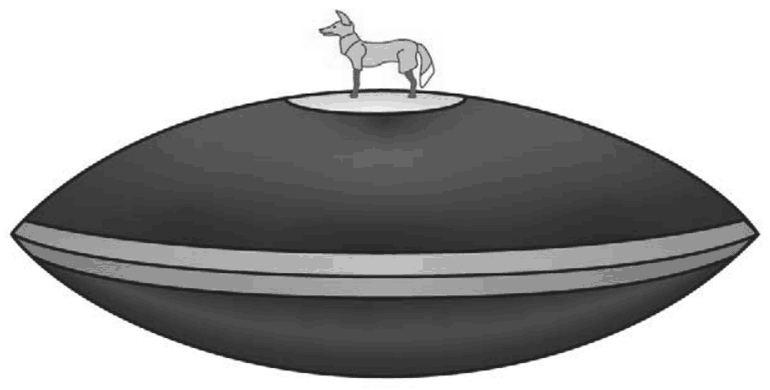
\includegraphics[width=0.42\linewidth]{enem2024_q131_mirascopio}\hfill
  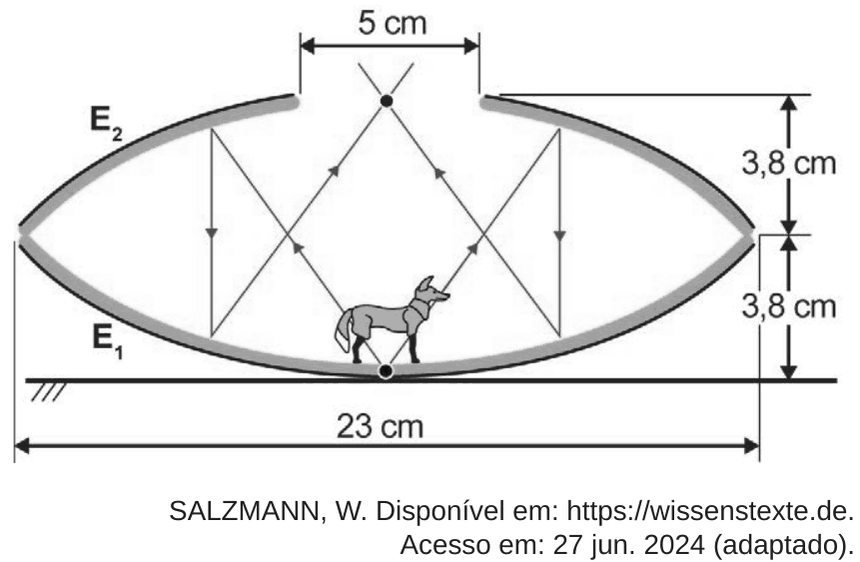
\includegraphics[width=0.5\linewidth]{enem2024_q131_esquema}
\end{center}

A natureza da imagem formada e a dist\^ancia vertical entre cada ponto objeto
e seu correspondente ponto imagem s\~ao
\begin{enumerate}
  \item real e 5 cm.
  \item real e 3,8 cm.
  \item real e 7,6 cm.
  \item virtual e 7,6 cm.
  \item virtual e 3,8 cm.
\end{enumerate}
\end{questao}

% ===================================================================
\newpage
\parte{Gabarito Comentado}
% ===================================================================

\begin{center}
{\renewcommand{\arraystretch}{1.25}
\begin{tabular}{cccccccccc}
  \toprule
  1 & 2 & 3 & 4 & 5 & 6 & 7 & 8 & 9 & 10 \\
  \midrule
  D & C & C & A & B & E & D & D & A & C \\
  \bottomrule
\end{tabular}\\[0.7em]
\begin{tabular}{cccc}
  \toprule
  11 & 12 & 13 & 14 \\
  \midrule
  E & E & D & C \\
  \bottomrule
\end{tabular}}
\end{center}

\medskip

\begin{description}[style=nextline, leftmargin=0pt]

\item[Q1 --- D (infravermelho e r\'adio).]
O controle da TV precisa de ``linha de visada'' e alcance curto: \'e
\textbf{infravermelho}, luz invis\'ivel que um obst\'aculo bloqueia. Para
quil\^ometros e contornando obst\'aculos, o drone usa \textbf{r\'adio}, de
comprimento de onda grande. Raios X e ultravioleta nem s\~ao usados em
controle remoto.

\item[Q2 --- C (a onda perde energia no caminho).]
Quanto mais longo o barbante, mais energia se dissipa: o som chega mais
fraco, ou seja, com menor \textbf{amplitude}. A frequ\^encia (e, com ela, a
altura e o per\'iodo) \'e da fonte e n\~ao muda; a velocidade e o comprimento
de onda dependem do meio, que continua o mesmo barbante.

\item[Q3 --- C (s\'o interfere o que tem a mesma frequ\^encia).]
O r\'adio do avi\~ao \'e sintonizado numa frequ\^encia; um sinal do celular s\'o
atrapalha se estiver nessa mesma frequ\^encia. Pot\^encia e intensidade n\~ao
bastam, e ondas eletromagn\'eticas nem s\~ao ``aud\'iveis'' (A). Todas se
propagam com a mesma velocidade no ar (E).

\item[Q4 --- A (menor $\lambda$, menos difra\c{c}\~ao).]
Cavidade menor exige luz de comprimento de onda menor para n\~ao difratar.
Entre as op\c{c}\~oes, o menor $\lambda$ do vis\'ivel \'e o \textbf{violeta}. \'E o
Blu-ray: 405 nm, contra 650 nm do DVD e 780 nm do CD.

\item[Q5 --- B (interfer\^encia destrutiva).]
O fone capta o ru\'ido e emite uma onda igual e \textbf{invertida}: crista
encontra vale e a soma se anula. Funciona para ru\'ido constante, como a
turbina, porque d\'a para prever a onda --- choro de beb\^e \'e irregular
demais.

\item[Q6 --- E (dois sinais que se cancelam).]
``Mesmo comprimento de onda'' e ``se cancelam'' \'e a defini\c{c}\~ao de
\textbf{interfer\^encia} destrutiva --- \'e a Q5 com outras palavras.
Resson\^ancia seria um sistema vibrando na pr\'opria frequ\^encia natural;
nada vibra aqui.

\item[Q7 --- D (barra curta, som agudo; mesmo material, mesma velocidade).]
A velocidade do som depende do \textbf{meio}: mesmo material e espessura,
$v_1 = v_2$. A barra menor vibra com comprimento de onda menor e, com a
mesma velocidade, frequ\^encia maior: $f_1 > f_2$. \'E por isso que
instrumentos pequenos s\~ao agudos.

\item[Q8 --- D (Doppler duas vezes).]
Fonte se aproximando: as frentes de onda se ``amontoam'' e o som fica
\textbf{mais agudo}. O radar tamb\'em sente Doppler: a onda refletida pela
ambul\^ancia que se aproxima volta com frequ\^encia \textbf{maior},
$f_r > f_0$ --- \'e assim que o radar mede velocidade.

\item[Q9 --- A (cor vista \'e a complementar da absorvida).]
O caroteno aparece amarelo-alaranjado. No c\'irculo de cores, o
complementar do amarelo-alaranjado \'e o lado oposto: \textbf{violeta e
azul}. \'E a mesma l\'ogica da clorofila: absorve azul e vermelho e sobra o
verde.

\item[Q10 --- C (bastonete sente a quantidade de luz).]
O enunciado d\'a a chave: bastonetes respondem ao \textbf{n\'umero} de f\'otons,
isto \'e, \`a intensidade. Bastonetes mais sens\'iveis percebem pouca luz: o
animal \textbf{enxerga bem no escuro}. Cor (A, B, E) \'e trabalho dos cones.

\item[Q11 --- E (a luz sai do peixe e desvia ao sair da \'agua).]
A luz vem do peixe e \textbf{refrata} ao passar da \'agua para o ar,
afastando-se da normal. O olho prolonga o raio em linha reta e v\^e o peixe
mais acima do que ele est\'a. B e D caem de cara: \textbf{o olho n\~ao emite
luz}.

\item[Q12 --- E (a \'agua desvia a luz para dentro da casa).]
O furo \'e muito maior que $\lambda$: n\~ao h\'a difra\c{c}\~ao relevante (A), e o
enunciado faz quest\~ao de dizer isso. A luz do Sol entra pela garrafa, muda
de meio (ar, pl\'astico, \'agua) e \'e desviada, espalhando-se pelo ambiente:
\textbf{refra\c{c}\~ao}.

\item[Q13 --- D (pupila pequena, raios quase paralelos ao eixo).]
Debaixo d'\'agua, a c\'ornea quase n\~ao refrata e o olho erra o foco. Com a
pupila fechada, s\'o entram raios quase paralelos ao eixo, que precisam de
\textbf{pouco desvio} para chegar ao lugar certo da retina. \'E o mesmo motivo
de apertar os olhos para enxergar melhor sem \'oculos.

\item[Q14 --- C (real e 7,6 cm).]
A imagem aparece ``flutuando'' na abertura, onde os raios \textbf{se cruzam
de verdade}: \'e \textbf{real}. O objeto est\'a no v\'ertice de E$_1$ (embaixo)
e a imagem, na abertura de E$_2$ (em cima). Pelo esquema, a dist\^ancia
vertical \'e $3{,}8 + 3{,}8 = 7{,}6$ cm --- leitura de figura, sem f\'ormula.

\end{description}

\bigskip

\begin{painel}
{\small\scshape\color{grafite}fontes}\par\smallskip
\small
\begin{itemize}[nosep, leftmargin=1.5em]
  \item \textbf{Quest\~oes do ENEM de 2020 a 2025}: enunciados transcritos dos
        cadernos do INEP em \texttt{Provas\_antigas\_ENEM/}; as figuras s\~ao
        recortes da arte original.
  \item \textbf{Gabarito do ENEM}: conferido com os \texttt{*\_GB\_*} do
        diret\'orio; as duas quest\~oes de 2024 com o gabarito do caderno
        cinza regular (o do diret\'orio \'e o da reaplica\c{c}\~ao).
\end{itemize}
\end{painel}

\end{document}
